\documentclass[showpacs, oneside, onecolumn, prl, amsmath, amssymb, nofootinbib, superscriptaddress, notitlepage]{revtex4-1}


\usepackage{cases}
\usepackage{amsmath}
\usepackage{amssymb}
\usepackage{amsfonts}
\usepackage{amssymb}
\usepackage{dcolumn}
\usepackage{bm}
\usepackage{bbm}
\usepackage{graphicx}
\usepackage{xcolor}
\usepackage{array}
\usepackage{subfigure}
\usepackage{hyperref}
\usepackage{multirow}
\usepackage{verbatim}

%%%%%%%%%%%%%%%%%%%%%%%%%%%%%%%%%%%%%%%%%%%%%%%%%%%%%%%%%%%%%%%%%%%%%%%%%%%%%%%%%%%
\newcommand{\bra}[1]{\langle #1\vert}
\newcommand{\ket}[1]{\vert #1\rangle}
\newcommand{\nn}{\nonumber \\}
\newcommand{\lag}{\langle}
\newcommand{\rag}{\rangle}
\newcommand{\cN}{{\cal N}}
\newcommand{\cA}{{\cal A}}
\newcommand{\gsim}{\mathrel{\hbox{\rlap{\lower.55ex \hbox {$\sim$}}
                   \kern-.3em \raise.4ex \hbox{$>$}}}}
\newcommand{\lsim}{\mathrel{\hbox{\rlap{\lower.55ex \hbox {$\sim$}}
                   \kern-.3em \raise.4ex \hbox{$<$}}}}

\newcommand\be{\begin{equation}}
\newcommand\ba{\begin{align}}
\newcommand\bas{\begin{align*}}
\newcommand\bt{\begin{table}}
\newcommand\bts{\begin{table*}}
\newcommand\bfig{\begin{figure}}
\newcommand\bfs{\begin{figure*}}
\newcommand\ee{\end{equation}}
\newcommand\ea{\end{align}}
\newcommand\et{\end{table}}
\newcommand\ets{\end{table*}}
\newcommand\efig{\end{figure}}
\newcommand\efs{\end{figure*}}
\newcommand\sothat{$\ \ \Rightarrow\ \ $}


\newcommand\blue{\textcolor{blue}}
\newcommand\gray{\textcolor{gray}}
\newcommand\red{\textcolor{red}}




\hypersetup{colorlinks=true,
            breaklinks=true,
            pdfstartview=Fit,
            linkcolor=blue,
            citecolor=green,
            urlcolor=blue}

\bibliographystyle{apsrev4-1}




%%%%%%%%%%%%%%%%%%%%%%%%%%%%%%%%%%%%%%%%%%%%%%%%%%%%%%%%%%%%%%%%%%%%%%%%%%%%%%%%%%%
\begin{document}
	
\title{Phys 512 Problem Set 1}


\author{JIAO Hao}

\maketitle
%%%%%%%%%%%%%%%%%%%%%%%%%%%%%%%%%%%%%%%%%%%%%%%%%%%%%%%%%%%%%%%%%%%%%%%%%%%%%%%%%%%



%%%%%%%%%%%%%%%%%%%%%%%%%%%%%%%%%%%%%%%%%%%%%%%%%%%%%%%%%%%%%%%%%%%%%%%%%%%%%%%%
\section{Problem 1}

\textbf{a) make the problem linear. }

\bas
z & -z_0=a((x-x_0)^2+(y-y_0)^2)\\
\Rightarrow\ \ z&=a((x-x_0)^2+(y-y_0)^2)+z_0\\
&=a(x^2-2xx_0+x_0^2+y^2-2yy_0+y_0^2)+z_0\\
&=(ax_0^2+ay_0^2+z_0)-2ax_0\cdot x-2ay_0\cdot y+a\cdot(x^2+y^2)\\
&=c_0+c_1 x+c_2 y+c_3(x^2+y^2)
\end{align*}

\bas
c_0&=ax_0^2+ay_0^2+z_0\\
c_1&=-2ax_0\\
c_2&=-2ay_0\\
c_3&=a
\end{align*}
So we have:
\bas
a&=c_3\\
x_0&=-c_1/2a\\
y_0&=-c_2/2a\\
z_0&=c_0-ax_0^2-ay_0^2
\end{align*}

~~~~

\textbf{b) Carry out the fit.}

- The new parameters are  [-1.51231182e+03, 4.53599028e-04, -1.94115589e-02, 1.66704455e-04]

- x0= -1.3604886221977293 

- y0= 58.22147608157934 

- z0= -1512.8772100367873 

- a= 0.00016670445477401342

\bfig
	\centering
	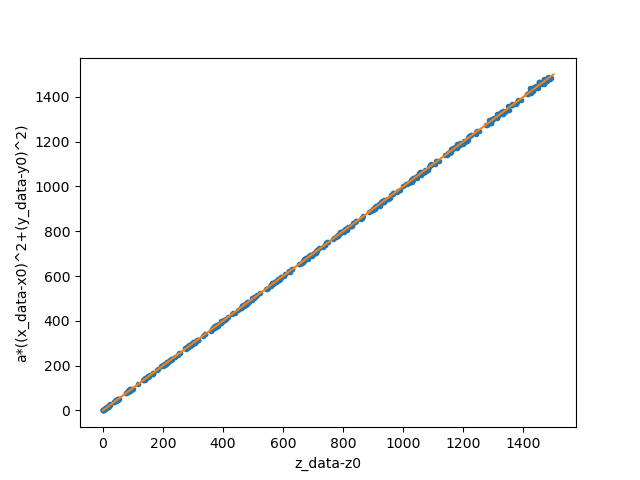
\includegraphics[scale=1]{3-1.png}
	\caption{Comparing $(z-z_0)$ and $a((x-x_0)^2+(y-y_0)^2)$. These points are from `dish\_zenith.txt', and the line corresponds to $(z-z_0)=a((x-x_0)^2+(y-y_0)^2)$.}
	\label{3-1}
\efig

From fig.\ref{3-1}, we can find that these parameters fit the data very well.

~~~~

\textbf{c) Estimate the noise and error}

The rms noise (np.std(r)) is 3.768338648784725, so $N=rms^2=14.200376171924686$.

Using the relation:
\bas
&N_{ij}=r_ir_j=(d-Am)_i(d-Am)_j\\
&R_{par}=(A^TN^{-1}A)^{-1}
\end{align*}
And the the uncertainty in a is equal to the (abs of) last eigenvalue of $R_{par}$. $\delta a\sim 7\times 10^{-33}$.

But here is a strange thing: if I set $r=z_{data}-Am$, the uncertainty is $-6.89\times 10^{-33}$, while if set $r=z_{data}-z_0-a((x_{data}-x_0)^2+(y_{data}-y_0)^2)$, the uncertainty becomes $-1.13\times10^{-33}$.

~~~~

The focal length
\bas
f&=1/4a\\
&\simeq 1499.7 (mm)\\
&=1.4997m
\end{align*}
The result is really closed to what we expect.

The error bar of f:
\bas
&f=\frac1{4a}\\
\Rightarrow\ \ &\ln f=-\ln(4a)=-\ln a-\ln4\\
\Rightarrow\ \ &\frac{df}{f}=-\frac{da}{a}\\
\Rightarrow\ \ &\delta f\sim \left|f\frac{\delta a}{a}\right|\simeq 6.2\times10^{-26}
\end{align*}

~~~~

\textbf{d) Check the circular symmetry of this system}

\bas
&x=\cos(\theta)x'+\sin(\theta)y',\ y=-\sin(\theta)x'+\cos(\theta)y'\\
\Rightarrow\ \ &x'=\cos(\theta)x-\sin(\theta)y,\ y'=\sin(\theta)x+\cos(\theta)y
\end{align*}
So we have
\bas
z-z_0'=&a(x'-x_0')^2+b(y'-y_0')^2\\
=&[ax_0^2+by_0^2]+[-2ax_0\cos(\theta)-2by_0\sin(\theta)]x+[a\cos^2(\theta)+b\sin^2(\theta)]x^2\\
&\ +[2(b-a)\cos(\theta)\sin(\theta)]xy+[2ax_0\sin(\theta)-2by_0\cos(\theta)]y+[a\sin^2(\theta)+b\cos^2(\theta)]y^2
\end{align*}

The result of the linear fitting is
\bas
\Rightarrow\ \ &c_0=ax_0^2+by_0^2=-1.51238281\times10^3\\
&c_1=-2ax_0\cos(\theta)-2by_0\sin(\theta)=4.19322347\times10^{-4}\\
&c_2=a\cos^2(\theta)+b\sin^2(\theta)=1.66414734\times10^{-4}\\
&c_3=2(b-a)\cos(\theta)\sin(\theta)=1.92159479\times10^{-6}\\
&c_4=2ax_0\sin(\theta)-2by_0\cos(\theta)=-1.93581475\times10^{-2}\\
&c_5=a\sin^2(\theta)+b\cos^2(\theta)=1.67074644e\times10^{-4}
\end{align*}

Solve the parameters:
\bas
&\theta=0.619999\,rad\\
&a=0.000165729\,mm^{-1}\\
&b=0.000167761\,mm^{-1}
\end{align*}
The focal lengths of the two principal axes are:
\bas
&f_a=1/4a\simeq 1.508m\\
&f_b=1/4b\simeq 1.490m
\end{align*}
The dish is not perfectly round, but almost round.

~~~~

~~~~

%%%%%%%%%%%%%%%%%%%%%%%%%%%%%%%%%%%%%%%%%%%%%%%%%%%%%%%%%%%%%%%%%%%%%%%%%%%%%%%%
\section{Problem 2}

The chi-square is 1588.4366720631901.

~~~~

~~~~

%%%%%%%%%%%%%%%%%%%%%%%%%%%%%%%%%%%%%%%%%%%%%%%%%%%%%%%%%%%%%%%%%%%%%%%%%%%%%%%%
\section{Problem 3}

Fix the optical depth, use Newton's method to find the best-fit values for the other parameters

~~~~

\textbf{output of this problem are:}

- The chi-square is 1588.4366720631901

- The  1 step take  31.9745614528656 sec to get the new parameters:

H0= 66.32313490629724 ,

ombh2= 0.022426531831128586 , omch2= 0.11757365503335179 ,

As= 2.0776196125643176e-09 , ns= 0.9642767515672348

The chi-square is 1238.7638191341052


- The  2 step take  31.048407316207886 sec to get the new parameters:

H0= 67.81467740180045 ,

ombh2= 0.022482342064984635 , omch2= 0.11653311269693893 ,

As= 2.0615773106630023e-09 , ns= 0.9685747818201237

The chi-square is 1228.9373523251652


- The  3 step take  30.891887187957764 sec to get the new parameters:

H0= 67.77395045784044 ,

ombh2= 0.022467707409121754 , omch2= 0.11658894563256587 ,

As= 2.0617920365457845e-09 , ns= 0.9682557435550914

The chi-square is 1228.9348815872177


- The  4 step take  33.107261657714844 sec to get the new parameters:

H0= 67.74490420650717 ,

ombh2= 0.022464389854556142 , omch2= 0.11664885855224674 ,

As= 2.062142071592309e-09 , ns= 0.9681325419094333

The chi-square is 1228.95062347248


- The  5 step take  32.4460015296936 sec to get the new parameters:

H0= 67.8313780177089 ,

ombh2= 0.022468154322113916 , omch2= 0.11643135994370327 ,

As= 2.0607686734715957e-09 , ns= 0.9684391092849786

The chi-square is 1228.9070552185162


- The  6 step take  33.036083459854126 sec to get the new parameters:

H0= 67.85642170543129 ,

ombh2= 0.022478491291904035 , omch2= 0.11641610874396584 ,

As= 2.0608237958190147e-09 , ns= 0.9686424066601074

The chi-square is 1228.9020655097295


- The  7 step take  31.852783679962158 sec to get the new parameters:

H0= 67.91537061534063 ,

ombh2= 0.02248517965604984 , omch2= 0.11628880453521921 ,

As= 2.060087891495517e-09 , ns= 0.9689019515466955

The chi-square is 1228.8780902854812


- The  8 step take  32.463271141052246 sec to get the new parameters:

H0= 67.9041321619901 ,

ombh2= 0.022480773343524288 , omch2= 0.11629313614028357 ,

As= 2.0600490365952568e-09 , ns= 0.9688176855522596

The chi-square is 1228.8831067191054


- The  9 step take  32.01904797554016 sec to get the new parameters:

H0= 67.85080459564647 ,

ombh2= 0.022471801683139257 , omch2= 0.11640409661029637 ,

As= 2.06065355949233e-09 , ns= 0.9685376496294616

The chi-square is 1228.8949275237655


- The  10 step take  32.23058581352234 sec to get the new parameters:

H0= 67.8753462432025 ,

ombh2= 0.0224797374072905 , omch2= 0.11636774179760019 ,

As= 2.060520942240872e-09 , ns= 0.9687158967380484

The final chi-square is 1228.8955015362942


- The step of the last step is 

dH0= 0.024541647556039995 ,

dombh2= 7.93572415124323e-06 , domch2= -3.635481269617146e-05 ,

dAs= -1.3261725145813479e-13 , dns= 0.00017824710858674683


- Error is  2493777018.643866


~~~~

Here I set the dpars=pars*1e-5 in the numerical derivative of spectrum. And I will show this assumption is reasonable at the end of this problem.

The chi-square of the last 6 steps are almost same (and $\Delta\chi^2<1$ after the second step), so I think the result is reliable. And the fitting is shown in fig.\ref{3-3}

\bfig
	\centering
	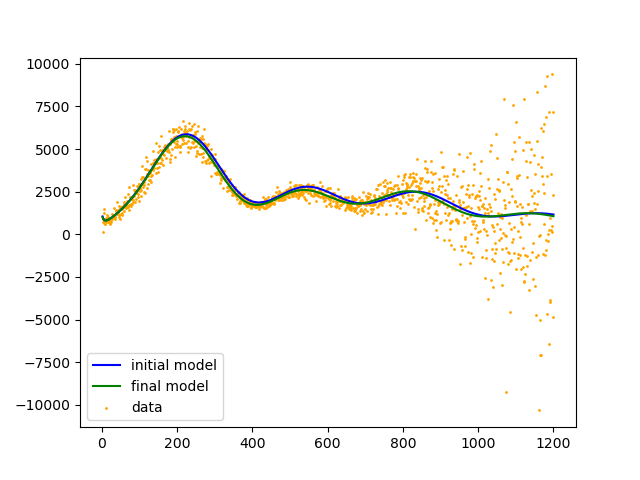
\includegraphics[scale=1]{3-3-1.png}
	\caption{Comparing the fitting of these parameters.}
	\label{3-3}
\efig





~~~~

Then, if we fix the other 5 parameters and only change tau:

\textbf{The output is:}

- The chi-square is 1228.8955015362942


- The 1 step take  13.377026796340942 sec to get the new parameters:

tau= 0.04998130669279882

The chi-square is 1228.8987549929382


- The 2 step take  12.990691900253296 sec to get the new parameters:

tau= 0.04998130661252405

The chi-square is 1228.8987550073566


- The 3 step take  13.550617218017578 sec to get the new parameters:

tau= 0.04998130661032868

The chi-square is 1228.8987550077516


- The 4 step take  13.935137271881104 sec to get the new parameters:

tau= 0.049981306610417116

The chi-square is 1228.898755007735


- The 5 step take  13.28310227394104 sec to get the new parameters:

tau= 0.049981306610951605

The chi-square is 1228.898755007639


- The 6 step take  13.573967218399048 sec to get the new parameters:

tau= 0.04998130661041387

The chi-square is 1228.8987550077359


- The 7 step take  13.582226276397705 sec to get the new parameters:

tau= 0.04998130661039576

The chi-square is 1228.898755007739


- The 8 step take  13.450579404830933 sec to get the new parameters:

tau= 0.049981306611026816

The chi-square is 1228.8987550076256


- The 9 step take  13.321529388427734 sec to get the new parameters:

tau= 0.04998130660970219

The chi-square is 1228.8987550078643


- The 10 step take  13.768777847290039 sec to get the new parameters:

tau= 0.04998130661140638

The final chi-square is 1228.8987550075572


- The step of the last step is 

dtau 1.704191718482376e-12


- Error is  2493776641.0844173

~~~~

The result is shown in fig.\ref{3-3-2}, the two fitting do not have obvious change!
\bfig
	\centering
	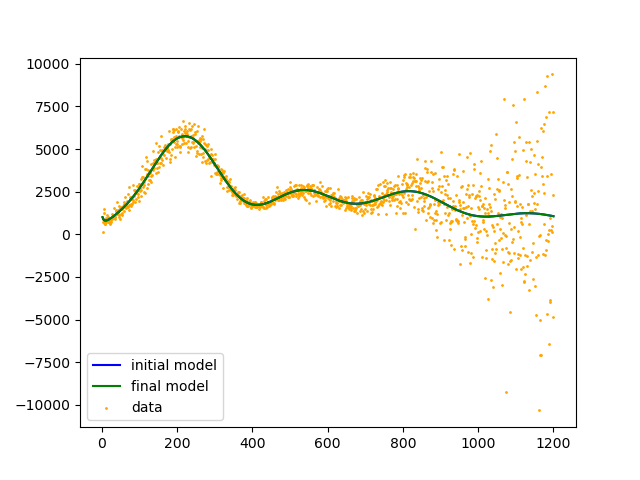
\includegraphics[scale=1]{3-3-2.png}
	\caption{Comparing the fitting of $\tau$.}
	\label{3-3-2}
\efig

~~~~

Finally, I will show that the numerical derivative of parameters of the above change dpars=pars*1e-5 is good enough to estimate the real derivative. I compared the numerical derivative of dpars=pars*1e-3, 1e-4 \& 1e-5 at the initial condition and the result are very similar (shown in fig.\ref{3-3-d}.

\bfig
	\centering
	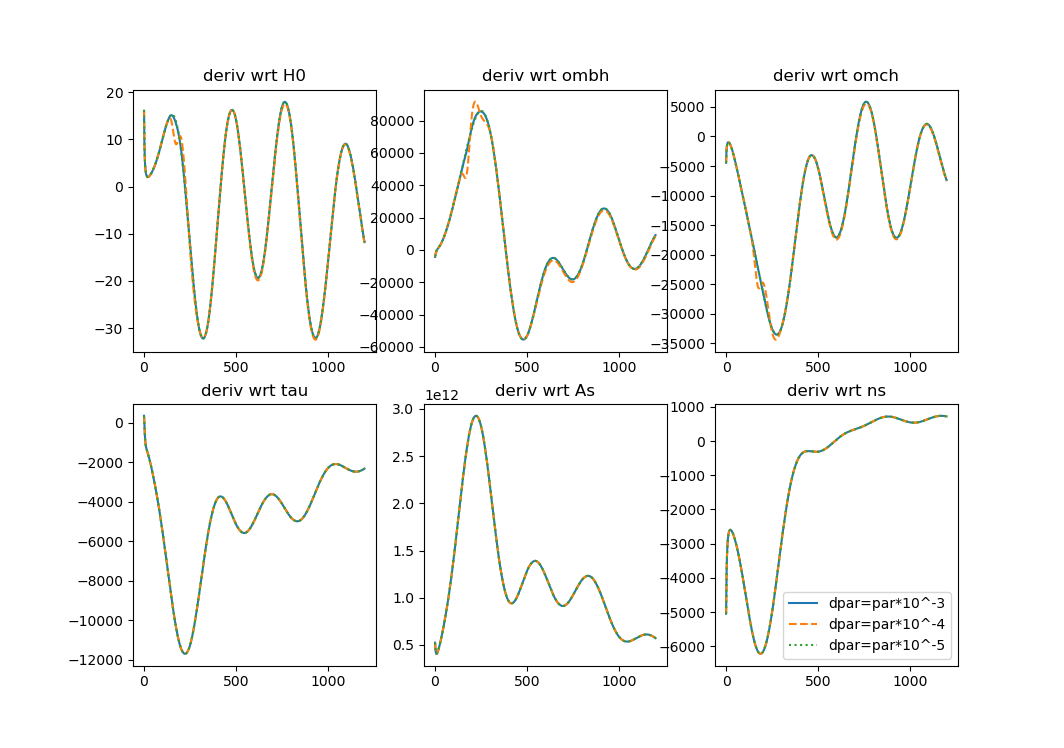
\includegraphics[scale=0.66]{3-3-3.png}
	\caption{Comparing the numerical derivative of every parameters.}
	\label{3-3-2}
\efig

~~~~

~~~~

%%%%%%%%%%%%%%%%%%%%%%%%%%%%%%%%%%%%%%%%%%%%%%%%%%%%%%%%%%%%%%%%%%%%%%%%%%%%%%%%
\section{Problem 4}

\bfig
	\centering
	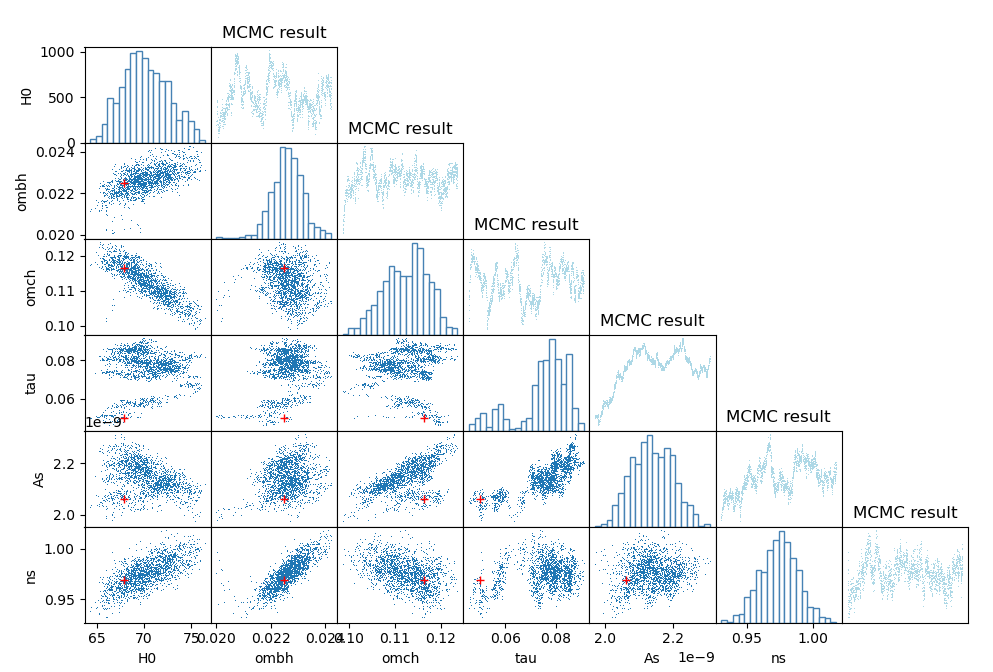
\includegraphics[scale=0.6]{3-4-1.png}
	\caption{MCMC simulation with $par\_step=par_0\times10^{-2}$. Red `+' denotes the parameters' value of the result of Newton's method.}
	\label{3-4-1}
\efig

\bfig
	\centering
	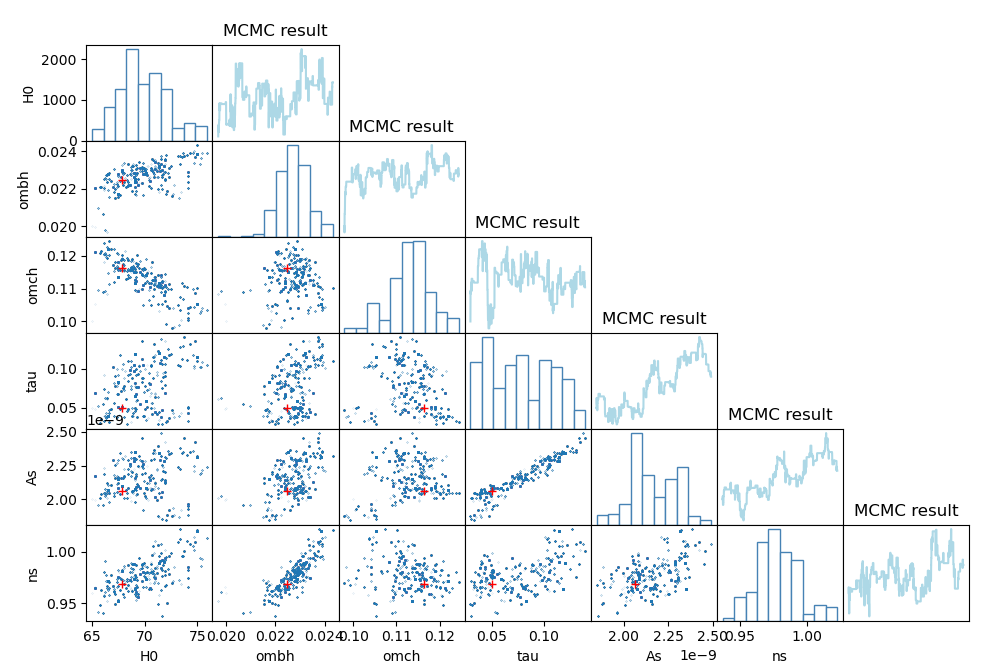
\includegraphics[scale=0.6]{3-4-2betterstep.png}
	\caption{MCMC simulation with $par\_step=np.std(par)$. Red `+' denotes the parameters' value of the result of Newton's method.}
	\label{3-4-2}
\efig

\bfig
	\centering
	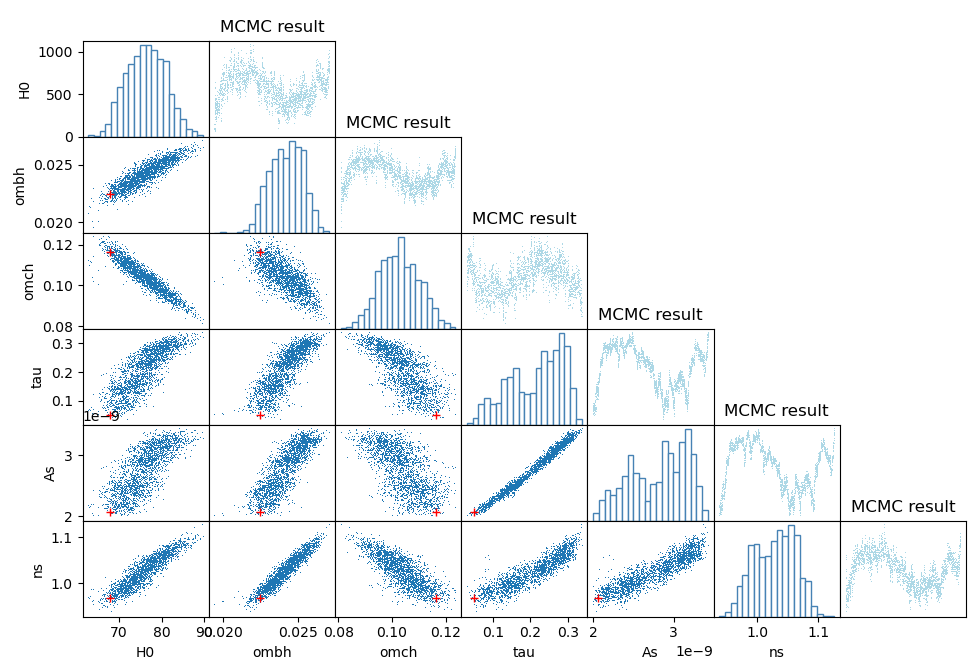
\includegraphics[scale=0.7]{3-4-3corr.png}
	\caption{MCMC simulation with correlated steps. Red `+' denotes the parameters' value of the result of Newton's method.}
	\label{3-4-3}
\efig

Here I set the initial parameters with the same value of \textbf{Problem 2}.

I first use the $par\_step=par_0\times 10^{-2}$, set nstep=10000. It shows that I get 1937 samples. The result of this MCMC simulation is shown in fig.\ref{3-4-1}. But the chain of this simulation does not like white noise and it seems the result is not very good.

So I then use two method taught in class to improve the simulation. The first is let the par\_step equal to the RMS of the chain (without the first 10\% steps). The result is shown in fig.\ref{3-4-2} and it seems even worse. I only get 197 steps, which means that the step is too large so I waste so many steps.

The third MCMC simulation uses the correlated steps and shown in fig.\ref{3-4-3}. I get 2375 samples, which is not much more than the first case. The correlation of parameters is very obvious but not very similar to the previous 2 cases. (I do not know why!) And also, the chain of this simulation does not like white noise. And what's strange is that the parameters' value get by Newton method are all in the edge of the possible area in parameter space.

\bfig
	\centering
	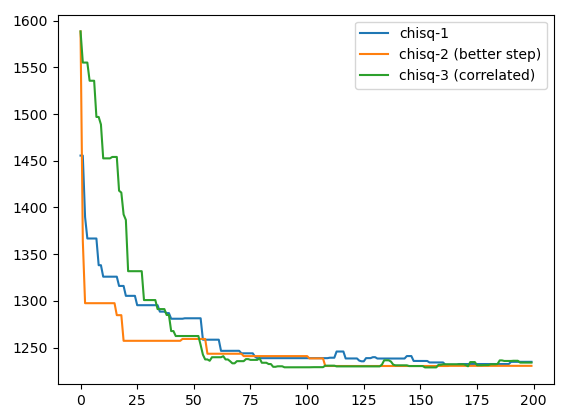
\includegraphics[scale=0.85]{3-4-chi(200).png}
	\caption{$\chi^2$ of the first 200 steps.}
	\label{3-4-4}
\efig

\bfig
	\centering
	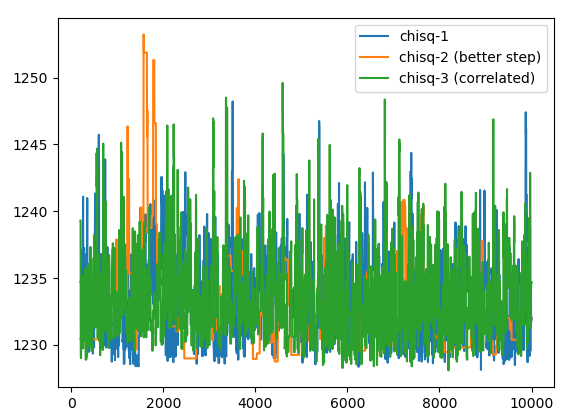
\includegraphics[scale=0.85]{3-4-chi(9800).png}
	\caption{$\chi^2$ of the latter steps.}
	\label{3-4-5}
\efig

The $\chi^2$ of the three simulations zre shown in fig.\ref{3-4-4} and \ref{3-4-5}

~~~~

\textbf{Then (since the deadline is extend and I have time to improve my simulation), I run a MCMC with 20,000 steps, this simulation fits much better!! The result for random step and correlated step are show in fig.\ref{3-4-1-20000} and \ref{3-4-3-20000}}

\bfig
	\centering
	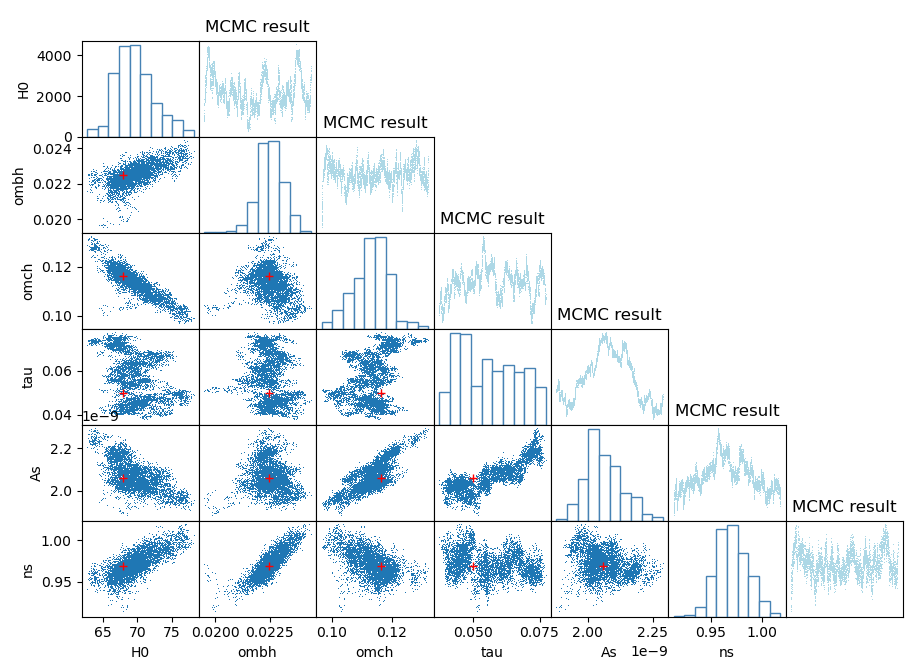
\includegraphics[scale=0.72]{3-4-1(20000).png}
	\caption{MCMC simulation with 20000 random steps. Red `+' denotes the parameters' value of the result of Newton's method.}
	\label{3-4-1-20000}
\efig

\bfig
	\centering
	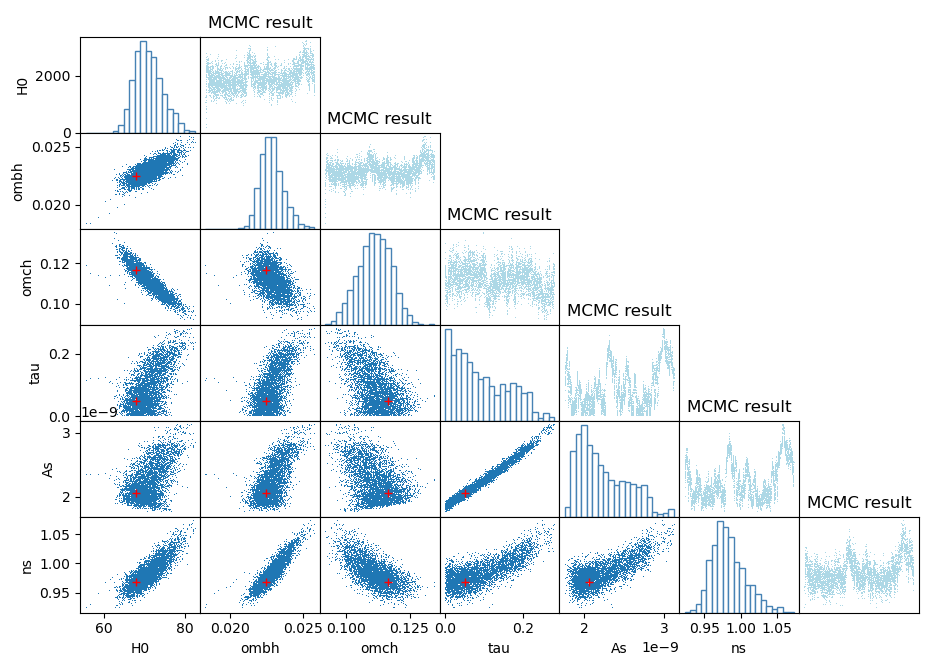
\includegraphics[scale=0.72]{3-4-3(20000).png}
	\caption{MCMC simulation with 20000 correlated steps.}
	\label{3-4-3-20000}
\efig

\bfig
	\centering
	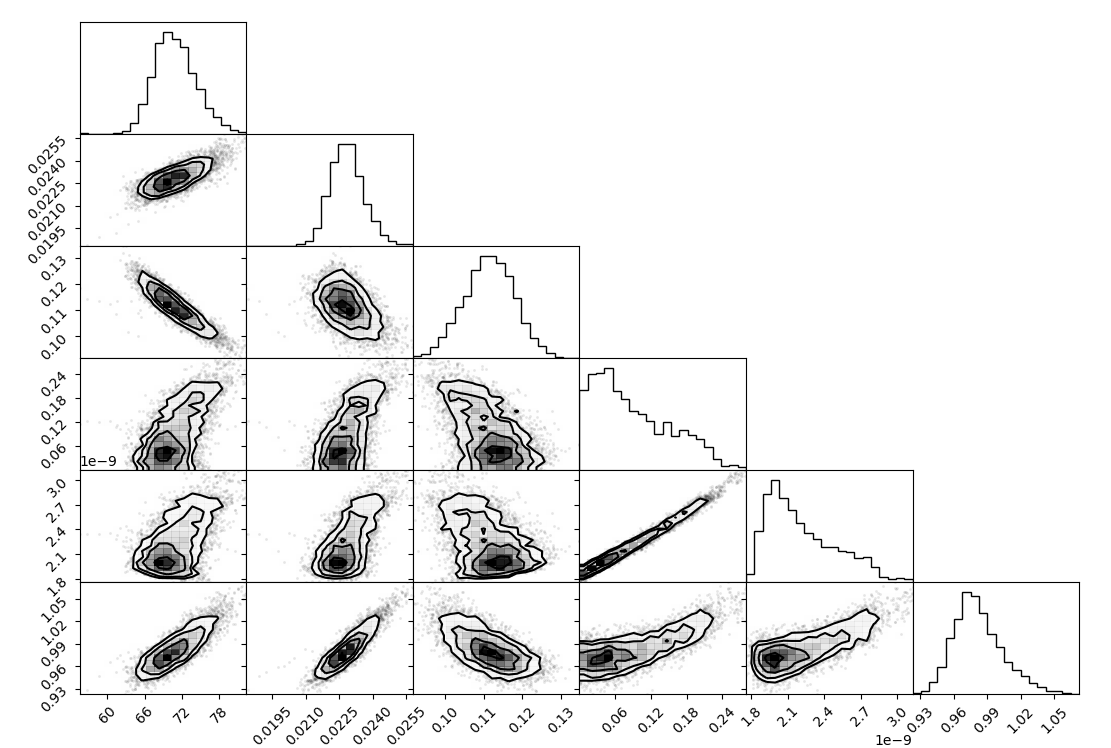
\includegraphics[scale=0.5]{3-4-3(20000)s.png}
	\caption{MCMC simulation with 4905 samples.}
	\label{3-4-6}
\efig

If I use `corner.corner()', the result of final case is shown in fig.\ref{3-4-6}.

~~~~

And the expected value of all parameters (from the last simulation) are:

From the last chain, the parameters are:

- H0= 7.10669497e+01 , 	    sigma\_H0= 3.39141641

- ombh= 2.28925106e-02 , 	sigma\_ombh= 7.77452523e-04

- omch= 1.11157293e-01 , 	sigma\_omch= 6.42114581e-03

- tau= 9.38460587e-02 , 	sigma\_tau= 6.93330159e-02

- As= 2.23683871e-09 , 		sigma\_As= 3.04510919e-10

- ns= 9.83609865e-01 , 	    sigma\_ns= 2.32742885e-02

~~~~

And the parameters obtained by the \textbf{sample} of last simulation is:

- H0= 7.09229544e+01 , 	    sigma\_H0= 3.34047650

- ombh= 2.28469019e-02 , 	sigma\_ombh= 7.64171305e-04

- omch= 1.11397389e-01 , 	sigma\_omch= 6.41296393e-03

- tau= 9.00203018e-02 , 	sigma\_tau= 6.41432411e-02

- As= 2.21821842e-09 , 		sigma\_As= 2.81833904e-10

- ns= 9.82268950e-01 , 	    sigma\_ns= 2.22798318e-02

~~~~

The two cases are very similar!

~~~~

~~~~

%%%%%%%%%%%%%%%%%%%%%%%%%%%%%%%%%%%%%%%%%%%%%%%%%%%%%%%%%%%%%%%%%%%%%%%%%%%%%%%%
\section{Problem 5}

Using `Importance Sampling' to deal with the sample get from the lasr simulation (20,000 \textbf{correlated} steps), I can get the expected value of all parameters:

- H0= 69.58494933919009 , 	    sigma\_H0= 2.3056820437899064

- ombh= 0.022560706054178377 , 	sigma\_ombh= 0.0007478180691303776

- omch= 0.11384070220523158 , 	sigma\_omch= 0.0037774632230811196

- tau= 0.05360145222357419 , 	sigma\_tau= 0.001796241854843383

- As= 2.058863059670732e-09 , 	sigma\_As= 6.828519672104872e-11

- ns= 0.971633499380878 , 	    sigma\_ns= 0.03219035346501125

Here the rms error is calculated by 
$$\sigma_x=\sqrt{\sum(x-\bar x)^2\times\text{prior}} / \sum \text{prior},$$
and I am not sure if this calculation is right.


~~~~

If I use the chain get from the 20,000 \textbf{random} steps simulation, the result will be:

- H0= 70.0928539790628 ,		sigma\_H0= 1.123856094279559

- ombh= 0.02245922516138705 ,	sigma\_ombh= 0.00035929530606787507

- omch= 0.11174727951100444 ,	sigma\_omch= 0.0017923924590661

- tau= 0.05386498265838653 ,	sigma\_tau= 0.0008697327686047654

- As= 2.0415029159243506e-09 ,	sigma\_As= 3.271767965170771e-11

- ns= 0.9709568243987166 ,		sigma\_ns= 0.015556829599214023




\end{document}